\documentclass[]{article}
\usepackage[utf8]{inputenc}
\usepackage{graphicx}
\usepackage[spanish]{babel}

%opening
\title{Red Neuronal usando un autómata celular y algoritmos genéticos }
\author{Cristopher Aldama Pérez}

\begin{document}

\maketitle

\begin{abstract}
	
	El objetivo es crear un automata celular capaz de simular una pequeña de neuronal, donde
	cada célula del automata representa una neurona que conectada a sus vecinas puede realizar
	computos simples.
	Para encontrar el estado inicial de dicho autómata, se hace uso de un algoritmo 
	genético, ya que este facilita encaminar  la búsqueda de dicho estado inicial
	en todo el espacio posible de soluciones.

\end{abstract}

\section{Neuronas y Vecindad}

Las células del autómata representan 6 tipos diferentes de  neuronas, a cada tipo le corresponde un estado
diferente con una función especifica, la vecindad es tipo Von Neumann.
Las reglas de transición entre estados están determinadas por el operador de mutación del algoritmo
genético y son probabilisticas.

\begin{figure}
\centering
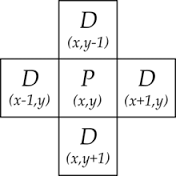
\includegraphics[width=0.4\linewidth]{von}
\caption{Vecindad Von Neumann}
\label{fig:von}
\end{figure}


\begin{tabular}{|c|c|c|}
	\hline Estado & Descripción & Color\\ 
	\hline Muerta & No transmite ni almacena información & Negro \\ 
	\hline Axón & Extrae información de neuronas vecinas & Verde \\ 
	\hline Dendrita & Transmite información a neuronas vecinas & Rojo \\ 
	\hline Cuerpo & Realiza computo de función de activación & Gris \\ 
	\hline Entrada & Extrae información del vector de Entrada & Azul \\ 
	\hline Salida & Guarda información al vector de salida & Amarillo \\ 
	\hline 
\end{tabular} 

Las neuronas de entrada leen directamente el vector de entrada y lo almacenan internamente para
su posterior transmisión por la red, en cambio las neuronas de salida toman los resultados
computados de sus vecinas y los escriben al vector de salida.

Las neuronas tipo Cuerpo, realizan el computo de la función de activación la cual es de tipo
sigmoide (\ref{eq:act}), para ello suman los valores internos de sus vecinas y el resultado lo aplican a la función de activación.


\begin{equation}\label{eq:act}
f(x) = \frac{1}{1 + {e^{x}}}
\end{equation}

\begin{equation}
x = \sum_{i=0}^{n} N_{i} 
\footnote{n: número de vecinos  }
\end{equation}


 

\section{Inicialización - Algoritmo Genético}
El estado inicial del autómata es buscado mediante el uso de un algoritmo genético, ya que este tipo de algoritmos permiten
llevar a cabo una búsqueda guiada por todas los estados iniciales posibles basándose en la prueba y error.
Todo el tablero está representado por una cadena de genes, donde a cada gen le corresponde una célula,
así si el tablero es de 10x10, el ADN que lo representa tiene longitud de 100. 
Cuando se hace una corrida se inicializan 20 individuos cada uno con su propio genoma, aunque en la interfaz solo muestre
el que mejor desempeño tiene.
Al inicio el genoma de cada individuo se iniciliza de manera aleatoria, y se le hacen pequeñas modificaciones o mutaciones 
en cada iteración con el fin de mejorar su desempeño a pasos pequeños.
Después de medir el desempeño de cada individuo, se selecciona a los 5 mejores, los cuales serán los
padres de la siguiente generación de individuos para así iniciar una nueva iteración.
Los resultados computados por el autómata  son comparados con los resultados esperados, así pues se obtiene un valor de error 
que representa la diferencia entre el valor esperado y el computado. El algoritmo genético esta diseñado para
minimizar esta diferencia.

\subsection{Genoma}

El Genoma de cada individuo esta codificado mediante una cadena de caracteres la cual indica el tipo de célula,
y su información inicial. Así pues fue necesario crear una función que creara células con datos aleatorios
para inicializar el genoma:

\begin{verbatim}
Board::Cell Board::Cell::fromRandom()
{
using Dist = std::uniform_int_distribution<int>;

static std::random_device rd;
static std::mt19937 gen(rd());
static Dist type(static_cast<int>(CellType::None), static_cast<int>(CellType::OUT));
static Dist dir(static_cast<int>(Direction::UP), static_cast<int>(Direction::NONE));

Cell c(static_cast<CellType>(type(gen)),
static_cast<Direction>(dir(gen)));
c.data = type(gen)/ 4.0;

return c;
}
\end{verbatim}

Y crear la cadena inicial

\begin{verbatim}
DNA initGenome(const size_t size)
{
DNA genes;

for(size_t i = 0; i < size; ++i){
auto g = Board::Cell::fromRandom();
genes.push_back(g);

}
return genes;
}
\end{verbatim}

\subsection{Mutación}

La mutación de los genes equivale a la transición entre estados de las células del autómata, y es meramente probabilistica,
las transiciones o estados elegidos durante la fase  de entrenamiento corresponden a aquellas configuraciones
que permitan al autómata realizar el computo de la función objetivo.

\begin{verbatim}
	void Board::Cell::mutate()
	{
	using int_dist = std::uniform_int_distribution<int>;
	static std::random_device dv;
	static std::mt19937 gen(dv());
	static int_dist dist_type (-m_amount_type, m_amount_type);
	static int_dist dist_dir (-m_amount_dir, m_amount_dir);
	
	int t = static_cast<int>(type);
	int d = static_cast<int>(dir);
	
	d += dist_dir(gen);
	t += dist_type(gen);
	
	if(t < 0){
	t = static_cast<int>(CellType::Body);
	}
	if(d < 0){
	d = static_cast<int>(Direction::NONE);
	}
	
	t = t % (static_cast<int>(CellType::Body) + 1);
	d = d % (static_cast<int>(Direction::NONE) + 1);
	
	type = static_cast<CellType>(t);
	dir = static_cast<Direction>(d);
	}
\end{verbatim}

\subsection{Función de Error}

La función de error esta definida como la diferencia entre el valor computado por el autómata el valor esperado del ejemplo.

\begin{equation}
e = min(\sum |y_{i} - c_{i}|)
\end{equation}

El objetivo es minimizar el error.

\section{Pruebas}

Para probar el autómata se tomaron las funciones booleanas OR y AND. Y se crearon automatas de 5x5, 10x10 y 100x100
para su calculo.

El autómata se inicializa con un estado inicial aleatorio, el cual va evolucionando de acuerdo a las reglas de transición dictadas 
por el algoritmo genético, se puede observar como se optimiza la función de error con forme pasan nuevas generaciones, hasta que el error
alcanza un valor de 0 y el autómata computa exitosamente la función booleana correspondiente.

\subsection{AND y OR}

\begin{figure}
\centering
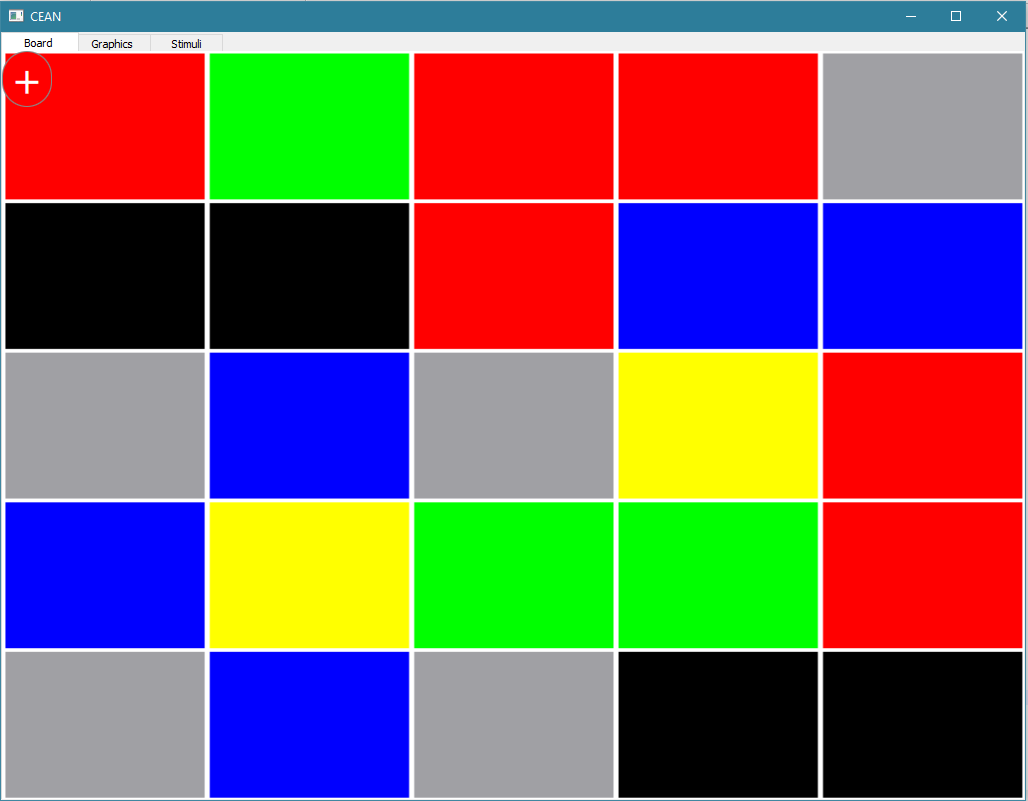
\includegraphics[width=0.7\linewidth]{or_estado}
\caption{Estado inicial 5x5}
\label{fig:or_estado}
\end{figure}


\begin{figure}
\centering
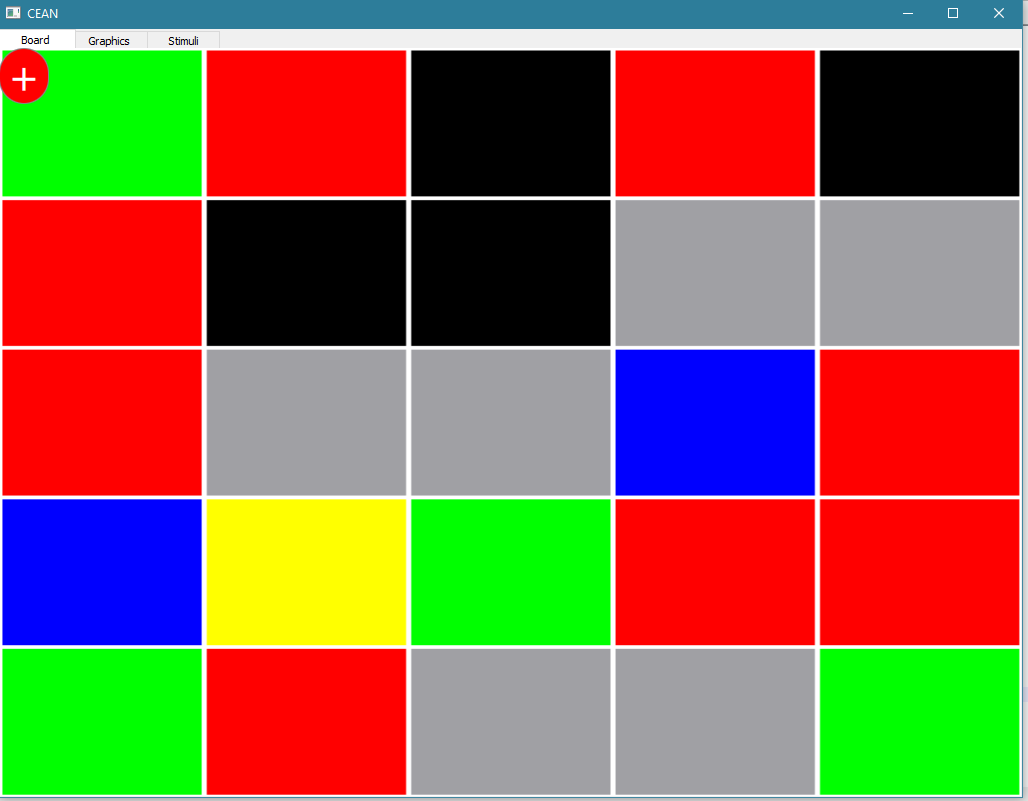
\includegraphics[width=0.7\linewidth]{or_estado_2}
\caption{Transiciones}
\label{fig:or_estado_2}
\end{figure}

\begin{figure}
\centering
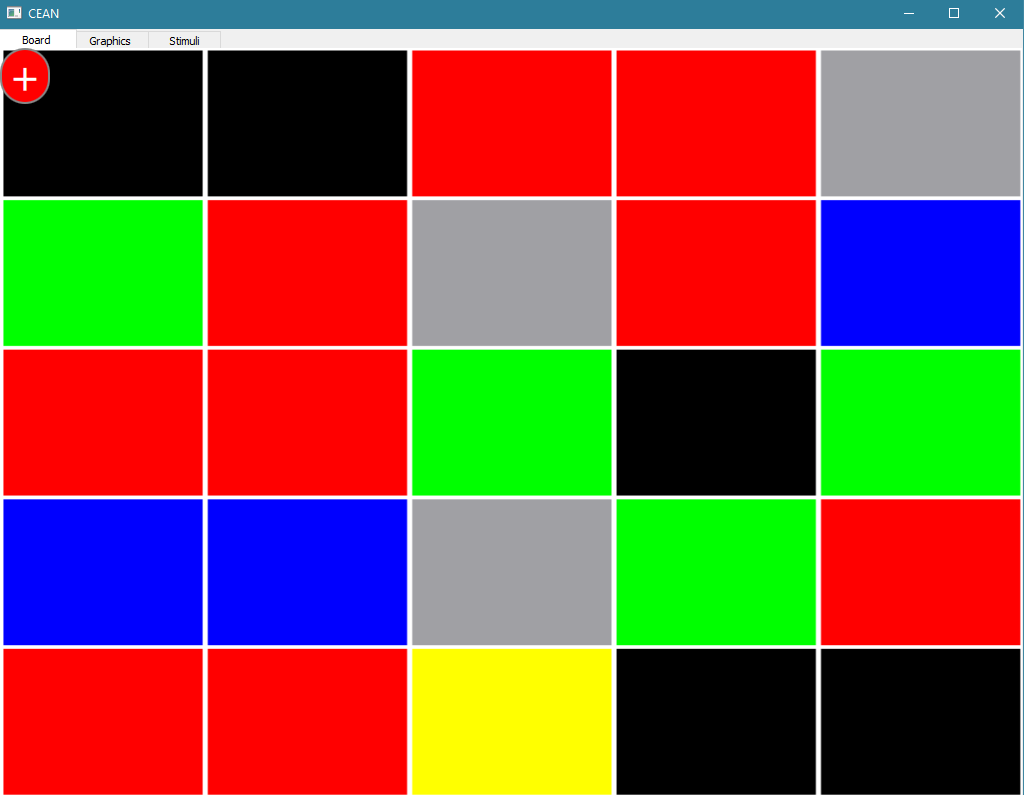
\includegraphics[width=0.7\linewidth]{or}
\caption{Atractor que computa exitosamente la función AND}
\label{fig:or_estado_2}
\end{figure}

\begin{figure}
\centering
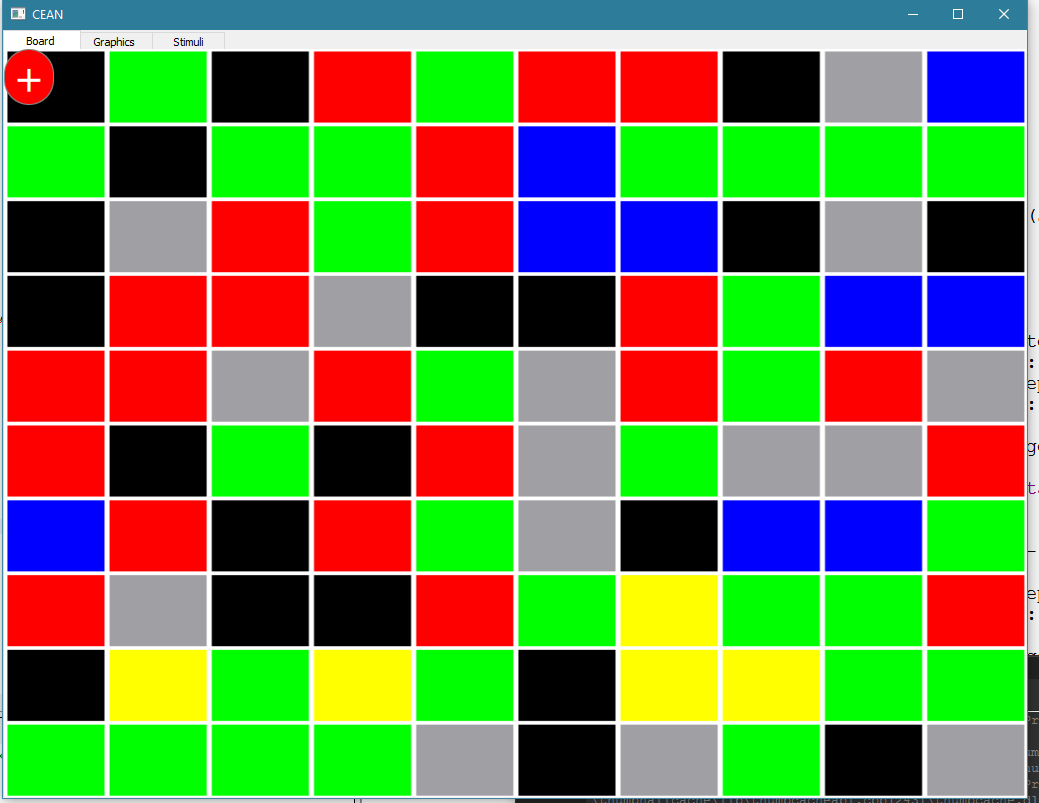
\includegraphics[width=0.7\linewidth]{or_1010}
\caption{Atractor que computa exitosamente la función AND (10x10)}
\label{fig:or_1010}
\end{figure}


\begin{figure}
	\centering
	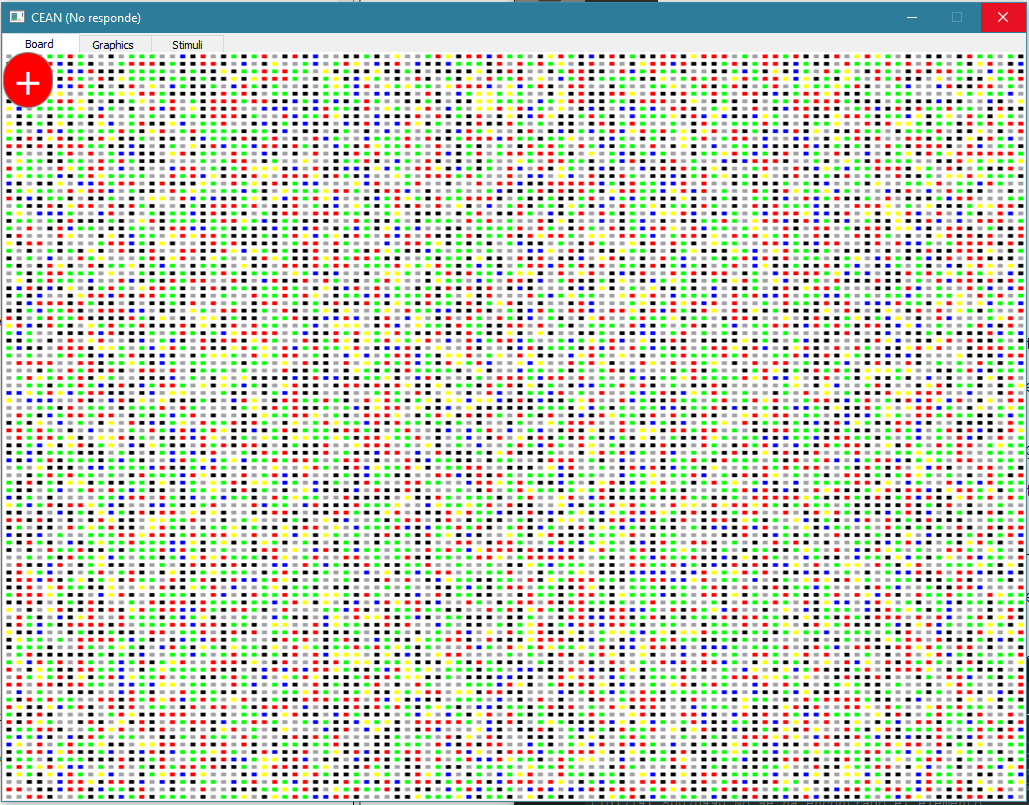
\includegraphics[width=0.7\linewidth]{or_100_100}
	\caption{Atractor que computa exitosamente la función AND (100x100)}
	\label{fig:or_1010}
\end{figure}
\begin{figure}
\centering
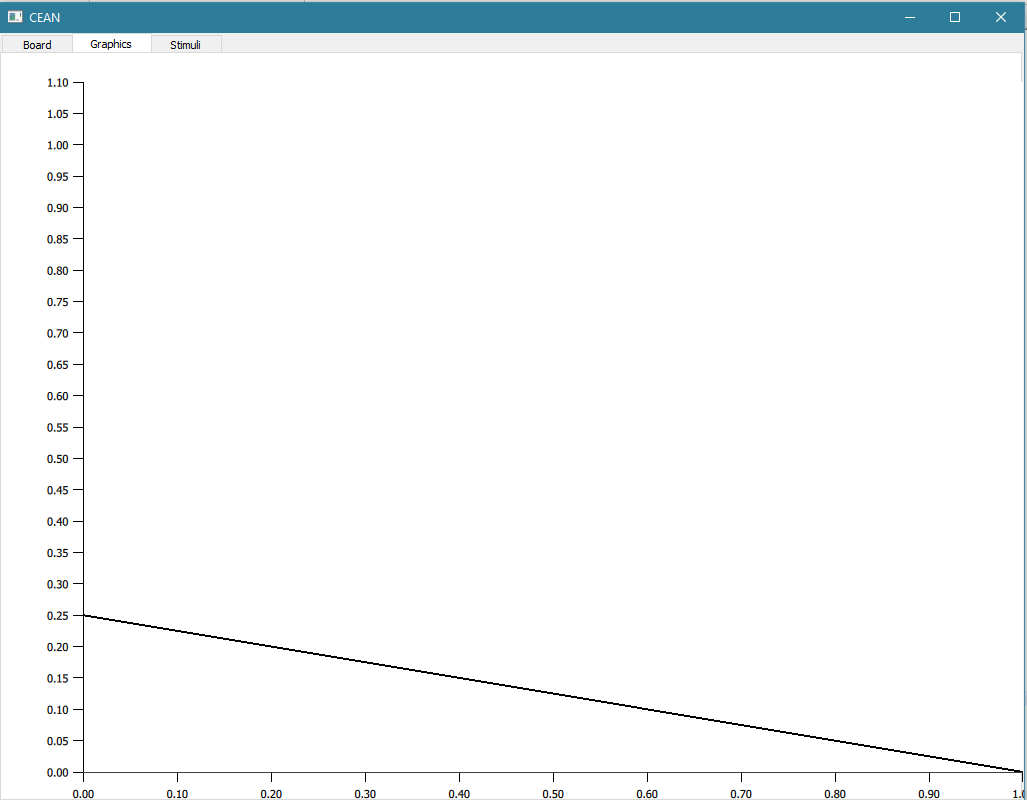
\includegraphics[width=0.7\linewidth]{or_error}
\caption{Minimización del error}
\label{fig:or_error}
\end{figure}

\begin{figure}
\centering
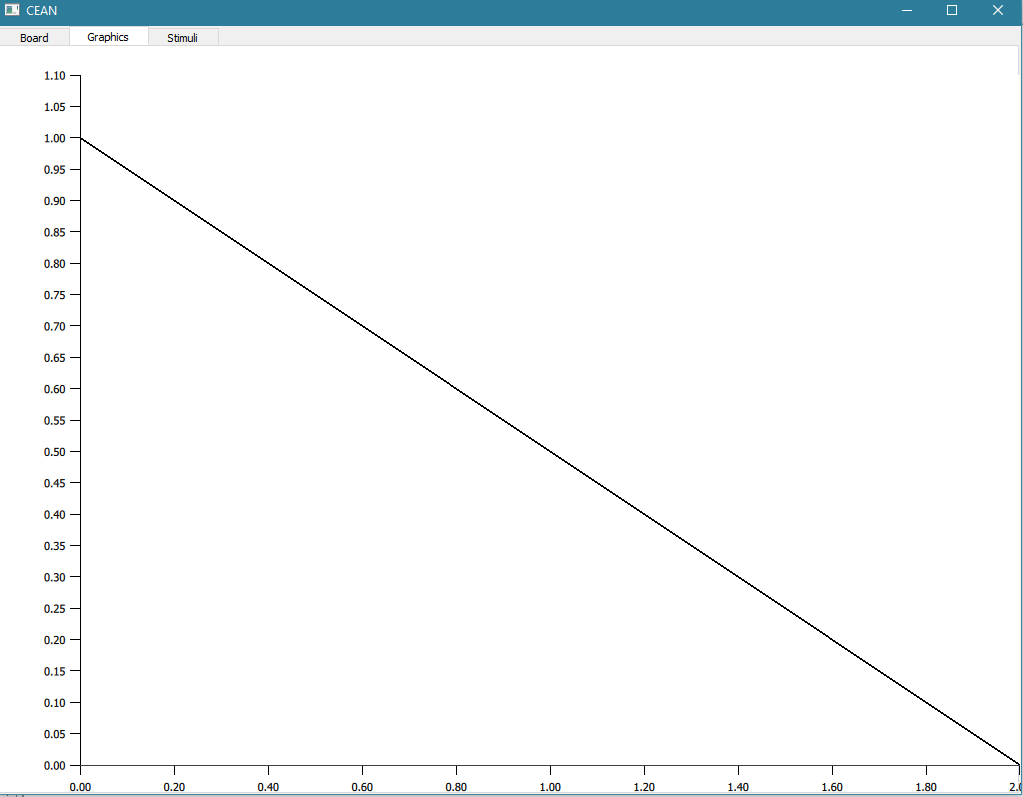
\includegraphics[width=0.7\linewidth]{or_error_2}
\caption{Minimización del error en corrida diferente}
\label{fig:or_error_2}
\end{figure}


\begin{figure}
\centering
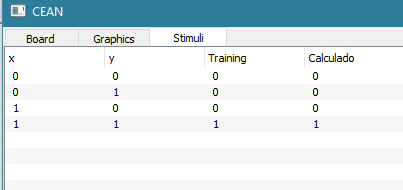
\includegraphics[width=0.7\linewidth]{or_salida}
\caption{computo de Función AND}
\label{fig:or_salida}
\end{figure}




\begin{figure}
\centering
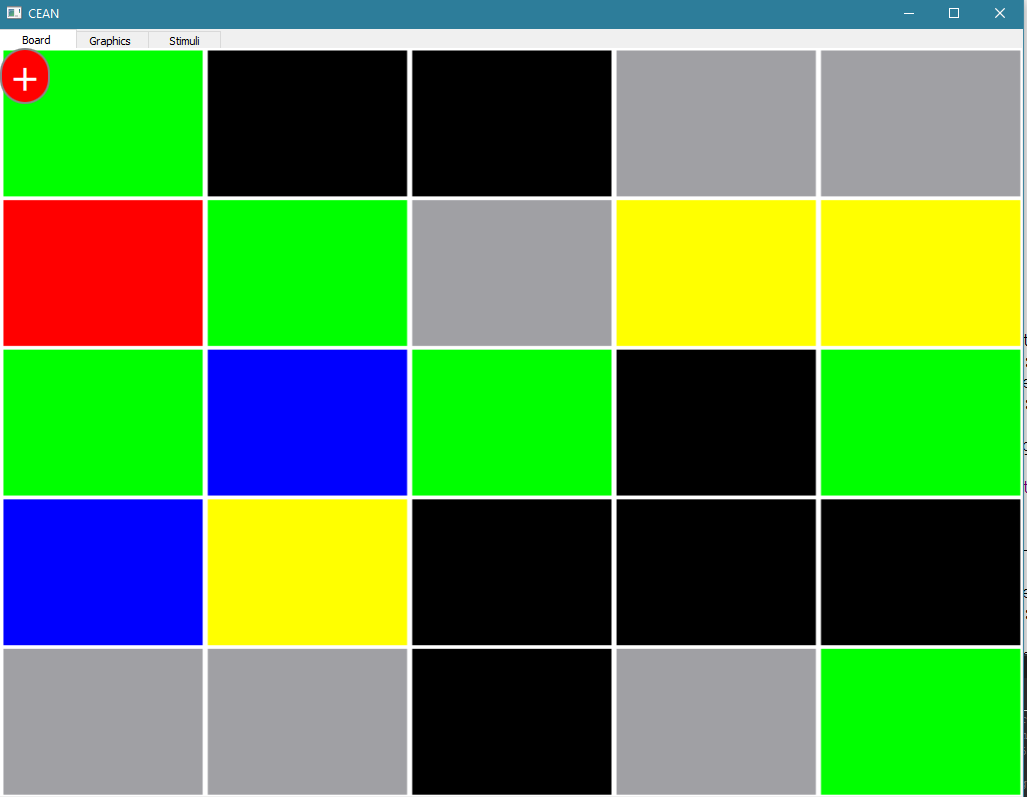
\includegraphics[width=0.7\linewidth]{ore_2}
\caption{Estado inicial aleatorio}
\label{fig:ore_2}
\end{figure}

\begin{figure}
\centering
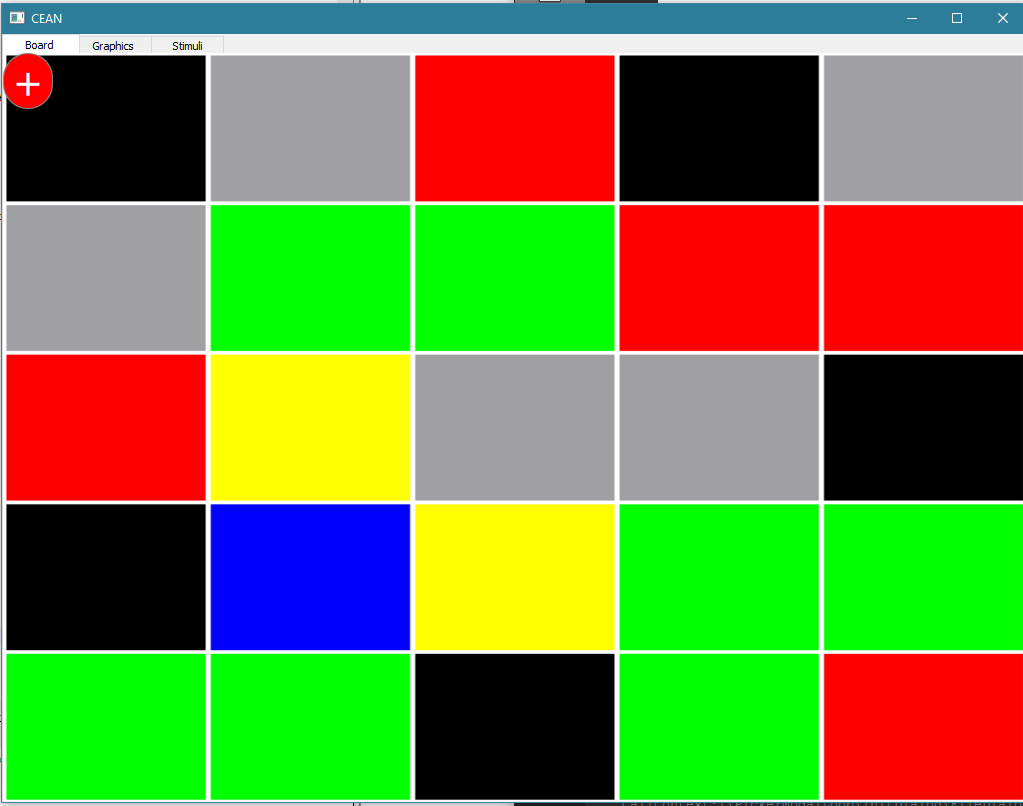
\includegraphics[width=0.7\linewidth]{ore}
\caption{Atractor que cómputa la función OR 5x5}
\label{fig:ore}
\end{figure}

\begin{figure}
\centering
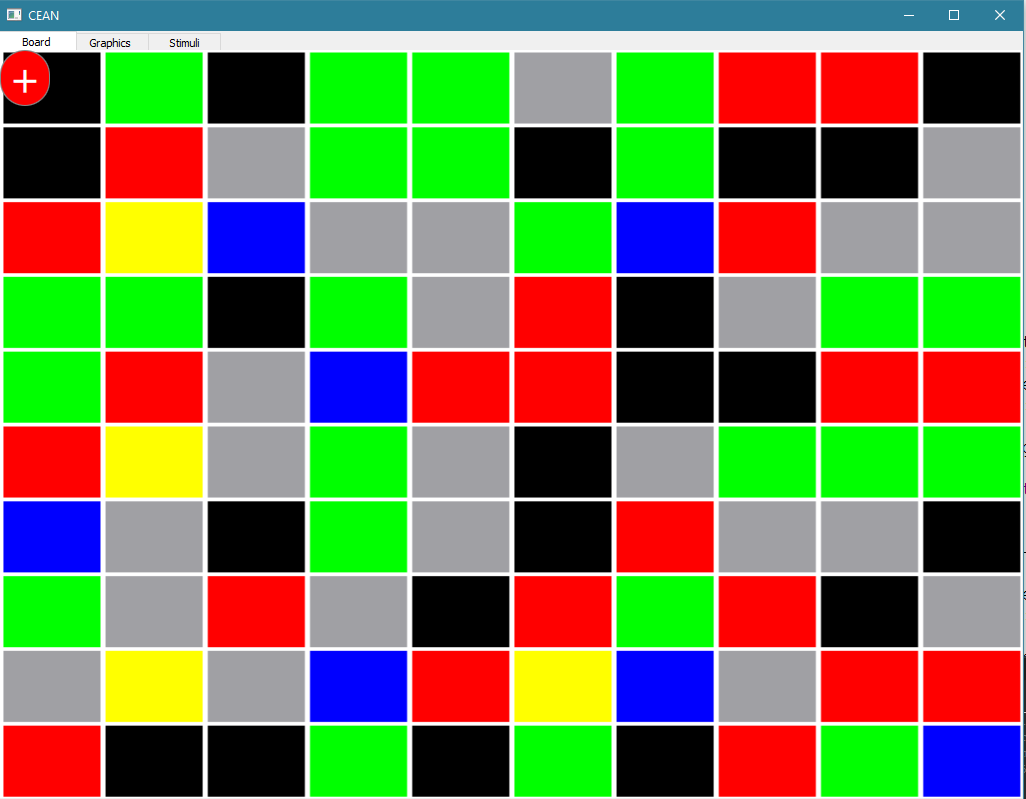
\includegraphics[width=0.7\linewidth]{ore_1010}
\caption{Atractor que cómputa la función OR 10x10}
\label{fig:ore_1010}
\end{figure}

\begin{figure}
\centering
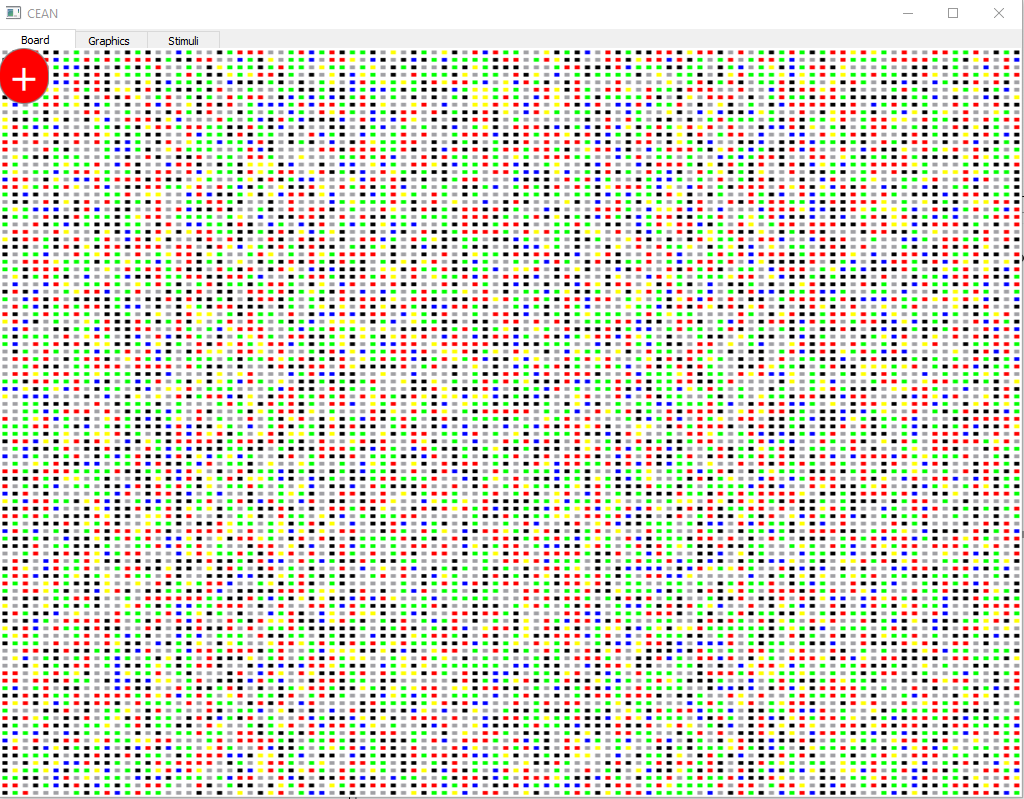
\includegraphics[width=0.7\linewidth]{ore100100}
\caption{Atractor que cómputa la función OR 100x100}
\label{fig:ore100100}
\end{figure}


\begin{figure}
\centering
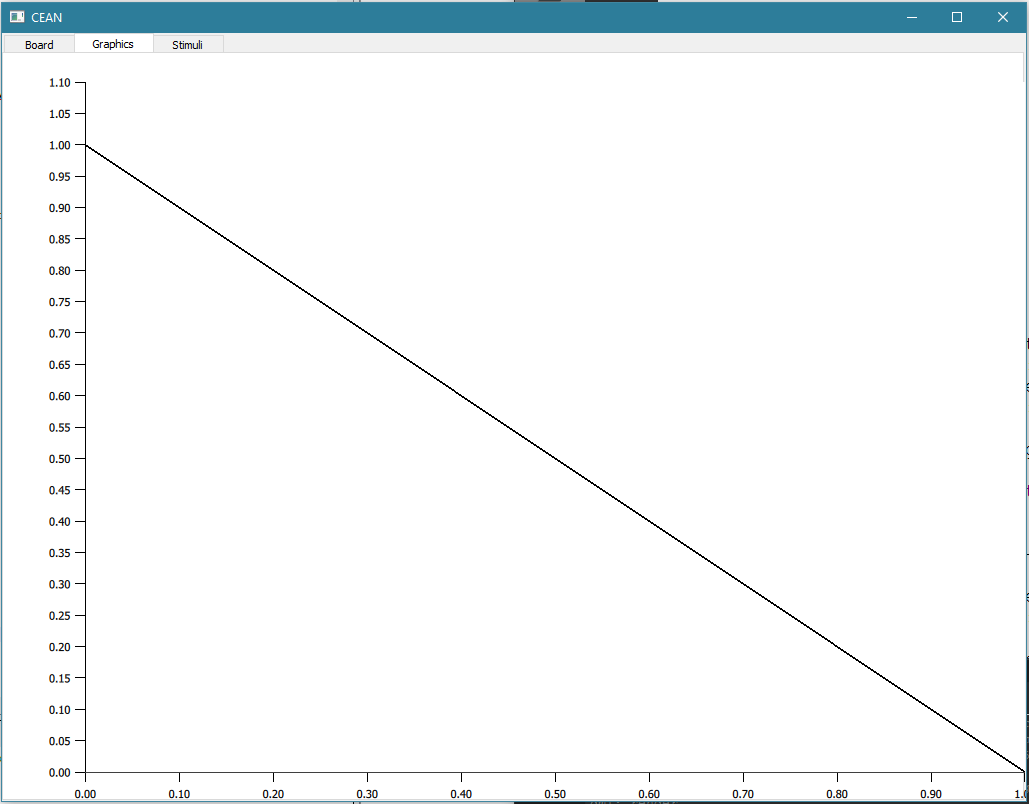
\includegraphics[width=0.7\linewidth]{ore_error}
\caption{Minimización de error}
\label{fig:ore_error}
\end{figure}

\begin{figure}
	\centering
	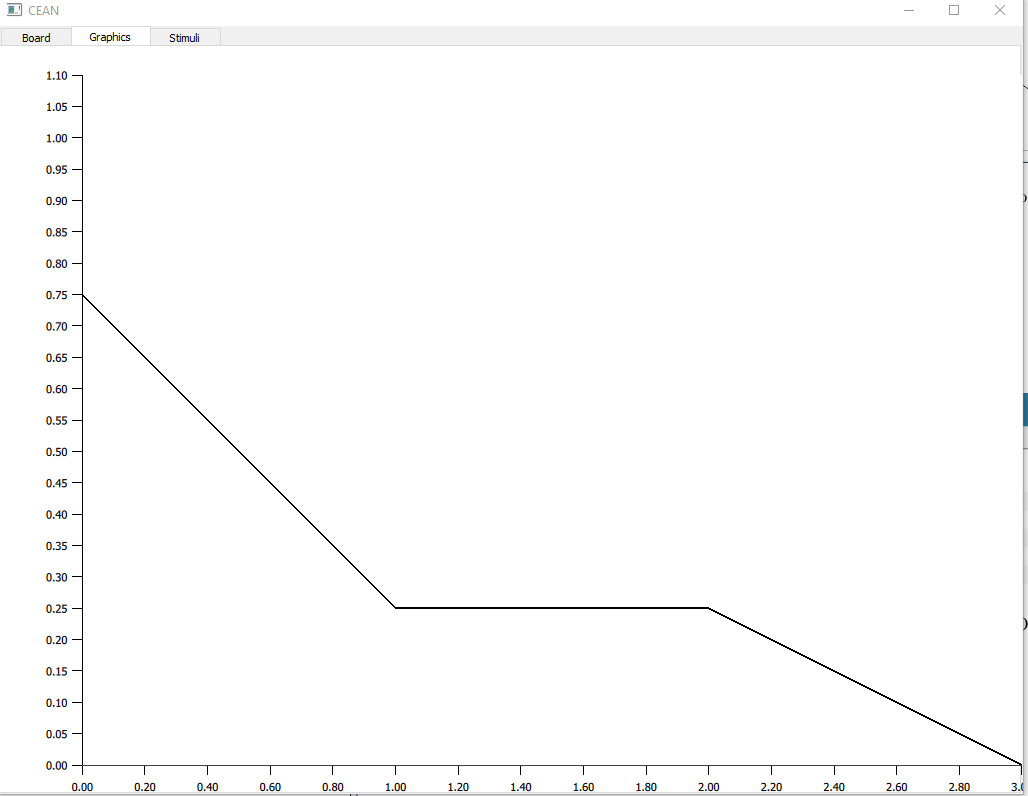
\includegraphics[width=0.7\linewidth]{ore_error_2}
	\caption{Minimización de error diferente corrida}
	\label{fig:ore_error}
\end{figure}

\begin{figure}
\centering
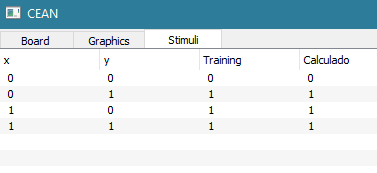
\includegraphics[width=0.7\linewidth]{ore_salida}
\caption{computo de función OR}
\label{fig:ore_salida}
\end{figure}







\end{document}
